\documentclass[12pt]{article}

% --- Packages ---
\usepackage{amsmath}
\usepackage{amssymb}
\usepackage{graphicx}
\usepackage{listings}
\usepackage{xcolor}
\usepackage{geometry}
\usepackage{hyperref}
\usepackage{enumitem}
\usepackage{caption}
\usepackage{dirtree}
\usepackage{booktabs}
\usepackage{array}
\usepackage{tikz}
\usepackage{tikz-3dplot}
\usepackage{textcomp}   % provides \textdegree outside math

\graphicspath{{./screenshots/}}
\geometry{margin=1in}
\setlength{\parindent}{0pt}
\setlength{\parskip}{6pt}
\setcounter{secnumdepth}{0}
\tolerance=1000
\emergencystretch=\maxdimen
\usetikzlibrary{arrows.meta}

% --- Code styling ---
\lstset{
    basicstyle=\ttfamily\small,
    keywordstyle=\color{blue},
    commentstyle=\color{gray},
    stringstyle=\color{orange},
    numbers=left,
    numberstyle=\tiny,
    breaklines=true,
    columns=fullflexible,   % prevents overfull hbox in listings
    frame=single,
    backgroundcolor=\color{gray!10}
}

\begin{document}

\begin{center}
    {\LARGE \textbf{RBE 500 -- Homework 3}} \\[6pt]
    {\large Tracy Yang} \\[4pt]
    {\large \today}
\end{center}

%=============================================================
\section{Part 1: Forward Kinematics / DH Parameters}

%-------------------------------------------------------------
\subsection{Task 1: Coordinate Frame Assignment (D-H Convention)}

Frames are assigned to the ABB IRB1400 as follows. All six joints are revolute.
\begin{itemize}
    \item \textbf{Frame 0 (base):} Fixed world frame. The $z_0$ axis
    points vertically upward along the axis of Joint~1. The origin $o_0$
    is at the base of the robot on the ground.

    \item \textbf{Frame 1:} Attached to the output of Joint~1.
    $z_1$ is aligned with the axis of Joint~2 (horizontal, perpendicular
    to the plane of the arm). The origin $o_1$ is 475\,mm above and
    150\,mm laterally offset from $o_0$.

    \item \textbf{Frame 2:} Attached to the output of Joint~2.
    $z_2$ is parallel to $z_1$. The link length $a_2 = 600$\,mm
    connects $o_1$ to $o_2$ along the upper arm.

    \item \textbf{Frame 3:} Attached to the output of Joint~3.
    $z_3$ is perpendicular to $z_2$, aligned with the axis of Joint~4.
    The link length $a_3 = 120$\,mm connects $o_2$ to $o_3$.

    \item \textbf{Frame 4:} Located at the center of the spherical
    wrist. $z_4$ is aligned with the axis of Joint~5.
    The offset $d_4 = 720$\,mm is the forearm length.

    \item \textbf{Frame 5:} Attached to Joint~5. $z_5$ is aligned
    with the axis of Joint~6, perpendicular to $z_4$.

    \item \textbf{Frame 6 (end-effector):} Located at the tip of the
    robot. $d_6 = 170 + 85 = 255$\,mm accounts for the wrist-to-tip
    distance (170\,mm wrist body + 85\,mm end-effector link).
\end{itemize}

\textbf{Assumptions:}
\begin{itemize}
    \item $z_0$ points vertically upward.
    \item The 150\,mm dimension is taken as the link offset $a_1$
    (perpendicular distance between $z_0$ and $z_1$).
    \item The home position corresponds to all joint variables
    $\theta_i = 0$.
    \item The total end-effector offset $d_6 = 170 + 85 = 255$\,mm
    combines the wrist body length and the end-effector link.
\end{itemize}

%-------------------------------------------------------------
\subsection{Task 2: D-H Parameter Table and Individual Transforms}

The standard D-H transformation from frame $i-1$ to frame $i$ is:
\[
T_i^{i-1} =
\begin{bmatrix}
    c\theta_i & -s\theta_i c\alpha_i &  s\theta_i s\alpha_i & a_i c\theta_i \\
    s\theta_i &  c\theta_i c\alpha_i & -c\theta_i s\alpha_i & a_i s\theta_i \\
    0         &  s\alpha_i           &  c\alpha_i           & d_i           \\
    0         &  0                   &  0                   & 1
\end{bmatrix}
\].

\begin{table}[h]
\centering
\caption{D-H Parameters for the ABB IRB1400 (all distances in mm)}
\renewcommand{\arraystretch}{1.3}
\begin{tabular}{ccccc}
\toprule
Joint $i$ & $\theta_i$ & $d_i$ (mm) & $a_i$ (mm) & $\alpha_i$ \\
\midrule
1 & $q_1$   & 475 & 150 & $+90^\circ$ \\
2 & $q_2$   &   0 & 600 &   $0^\circ$ \\
3 & $q_3$   &   0 & 120 & $+90^\circ$ \\
4 & $q_4$   & 720 &   0 & $-90^\circ$ \\
5 & $q_5$   &   0 &   0 & $+90^\circ$ \\
6 & $q_6$   & 255 &   0 &   $0^\circ$ \\
\bottomrule
\end{tabular}
\end{table}

\textbf{Individual transformation matrices}:

\[
T_1^0 =
\begin{bmatrix}
    c_1 & 0 &  s_1 & 150\,c_1 \\
    s_1 & 0 & -c_1 & 150\,s_1 \\
    0   & 1 &  0   & 475      \\
    0   & 0 &  0   & 1
\end{bmatrix}
\qquad
T_2^1 =
\begin{bmatrix}
    c_2 & -s_2 & 0 & 600\,c_2 \\
    s_2 &  c_2 & 0 & 600\,s_2 \\
    0   &  0   & 1 & 0        \\
    0   &  0   & 0 & 1
\end{bmatrix}
\]

\[
T_3^2 =
\begin{bmatrix}
    c_3 & 0 &  s_3 & 120\,c_3 \\
    s_3 & 0 & -c_3 & 120\,s_3 \\
    0   & 1 &  0   & 0        \\
    0   & 0 &  0   & 1
\end{bmatrix}
\qquad
T_4^3 =
\begin{bmatrix}
    c_4 &  0 & -s_4 & 0   \\
    s_4 &  0 &  c_4 & 0   \\
    0   & -1 &  0   & 720 \\
    0   &  0 &  0   & 1
\end{bmatrix}
\]

\[
T_5^4 =
\begin{bmatrix}
    c_5 & 0 &  s_5 & 0 \\
    s_5 & 0 & -c_5 & 0 \\
    0   & 1 &  0   & 0 \\
    0   & 0 &  0   & 1
\end{bmatrix}
\qquad
T_6^5 =
\begin{bmatrix}
    c_6 & -s_6 & 0 & 0   \\
    s_6 &  c_6 & 0 & 0   \\
    0   &  0   & 1 & 255 \\
    0   &  0   & 0 & 1
\end{bmatrix}
\]

%-------------------------------------------------------------
\subsection{Task 3: Composite Forward Kinematics}

The composite transformation from the base frame to the end-effector is:
\[
H = T_6^0 = T_1^0 \cdot T_2^1 \cdot T_3^2 \cdot T_4^3 \cdot T_5^4 \cdot T_6^5
\]

This was computed numerically in MATLAB using the function below.
The general symbolic form is a $4\times4$ matrix whose upper-left
$3\times3$ block encodes the end-effector orientation and whose
right-most column encodes the end-effector position in the base frame.

\begin{lstlisting}[language=Matlab,
    caption={MATLAB function: standard DH matrix}]
function T = dh_matrix(theta, d, a, alpha)
    % Returns the standard DH homogeneous transformation matrix.
    % Inputs: theta, alpha in degrees; d, a in mm.
    theta = deg2rad(theta);
    alpha = deg2rad(alpha);
    ct = cos(theta); st = sin(theta);
    ca = cos(alpha); sa = sin(alpha);
    T = [ct, -st*ca,  st*sa, a*ct;
         st,  ct*ca, -ct*sa, a*st;
          0,     sa,     ca,    d;
          0,      0,      0,    1];
end
\end{lstlisting}

\begin{lstlisting}[language=Matlab,
    caption={MATLAB function: IRB1400 forward kinematics}]
function [T, frames] = fk_irb1400(q)
    % Computes FK for the ABB IRB1400 using standard DH convention.
    % Input:  q = [q1, q2, q3, q4, q5, q6] in degrees
    % Output: T     = 4x4 end-effector pose in base frame
    %         frames = cell array of cumulative transforms {T0, T1, ..., T6}

    % DH table columns: [theta_i, d_i, a_i, alpha_i]
    dh = [q(1), 475, 150,  90;   % Joint 1: base rotation
          q(2),   0, 600,   0;   % Joint 2: shoulder
          q(3),   0, 120,  90;   % Joint 3: elbow
          q(4), 720,   0, -90;   % Joint 4: wrist 1
          q(5),   0,   0,  90;   % Joint 5: wrist 2
          q(6), 255,   0,   0];  % Joint 6: wrist 3 + EE

    T = eye(4);
    frames = {T};
    for i = 1:6
        Ti = dh_matrix(dh(i,1), dh(i,2), dh(i,3), dh(i,4));
        T  = T * Ti;
        frames{end+1} = T;
    end
end
\end{lstlisting}

%-------------------------------------------------------------
\subsection{Question 5: FK for Given Joint Configuration}

For $[\theta_1,\,\theta_2,\,\theta_3,\,\theta_4,\,\theta_5,\,\theta_6]
= [0^\circ,\;75^\circ,\;30^\circ,\;135^\circ,\;-45^\circ,\;60^\circ]$, the composite transformation
$H = T_6^0$ evaluates to:

\[
H =
\begin{bmatrix}
 0.5647 & -0.6121 &  0.5536 & 1110.87 \\
 0.3624 &  0.7866 &  0.5000 &  127.50 \\
-0.7415 & -0.0817 &  0.6660 & 1526.64 \\
 0      &  0      &  0      &  1
\end{bmatrix}
\]

\textbf{Position forward kinematics}
(end-effector origin expressed in the base frame, in mm):
\[
\mathbf{p} =
\begin{bmatrix} 1110.87 \\ 127.50 \\ 1526.64 \end{bmatrix} \text{ mm}
\]

\textbf{Orientation forward kinematics}
(rotation matrix from end-effector frame to base frame):
\[
R_6^0 =
\begin{bmatrix}
 0.5647 & -0.6121 &  0.5536 \\
 0.3624 &  0.7866 &  0.5000 \\
-0.7415 & -0.0817 &  0.6660
\end{bmatrix}
\]

The columns of $R_6^0$ give the directions of $x_6$, $y_6$, $z_6$
expressed in the base frame.

%-------------------------------------------------------------
\subsection{Question 6: MATLAB 3D Visualization}

\begin{lstlisting}[language=Matlab,
    caption={MATLAB robot visualization (draw\_irb1400.m)}]
function draw_irb1400(q)
    % Draws ABB IRB1400 in 3D based on joint configuration.
    % Input: q = [q1,..,q6] in degrees.
    % At q = [0,0,0,0,0,0] robot is at defined home position.

    % Compute forward kinematics and extract all frame origins
    [~, frames] = fk_irb1400(q);
    n = length(frames);
    positions = zeros(3, n);
    for i = 1:n
        positions(:, i) = frames{i}(1:3, 4);
    end

    figure; clf; hold on; grid on; axis equal;
    xlabel('X (mm)'); ylabel('Y (mm)'); zlabel('Z (mm)');
    title(sprintf('ABB IRB1400  q = [%s] deg', num2str(q, '%.0f ')));
    view(45, 20);

    % Draw links as thick solid lines
    plot3(positions(1,:), positions(2,:), positions(3,:), ...
          'b-', 'LineWidth', 3);

    % Draw joint origins as solid red circles
    plot3(positions(1,:), positions(2,:), positions(3,:), ...
          'ro', 'MarkerSize', 10, 'MarkerFaceColor', 'r');

    % Label each frame origin
    labels = {'o_0','o_1','o_2','o_3','o_4','o_5','o_6'};
    for i = 1:n
        text(positions(1,i)+20, positions(2,i)+20, positions(3,i)+20, ...
             labels{i}, 'FontSize', 9, 'FontWeight', 'bold');
    end
end

% ---- Run both configurations ----
figure(1); draw_irb1400([0, 0, 0, 0, 0, 0]);        % home
figure(2); draw_irb1400([0, 75, 30, 135, -45, 60]);  % question 5
\end{lstlisting}

\begin{figure}[h]
    \centering
    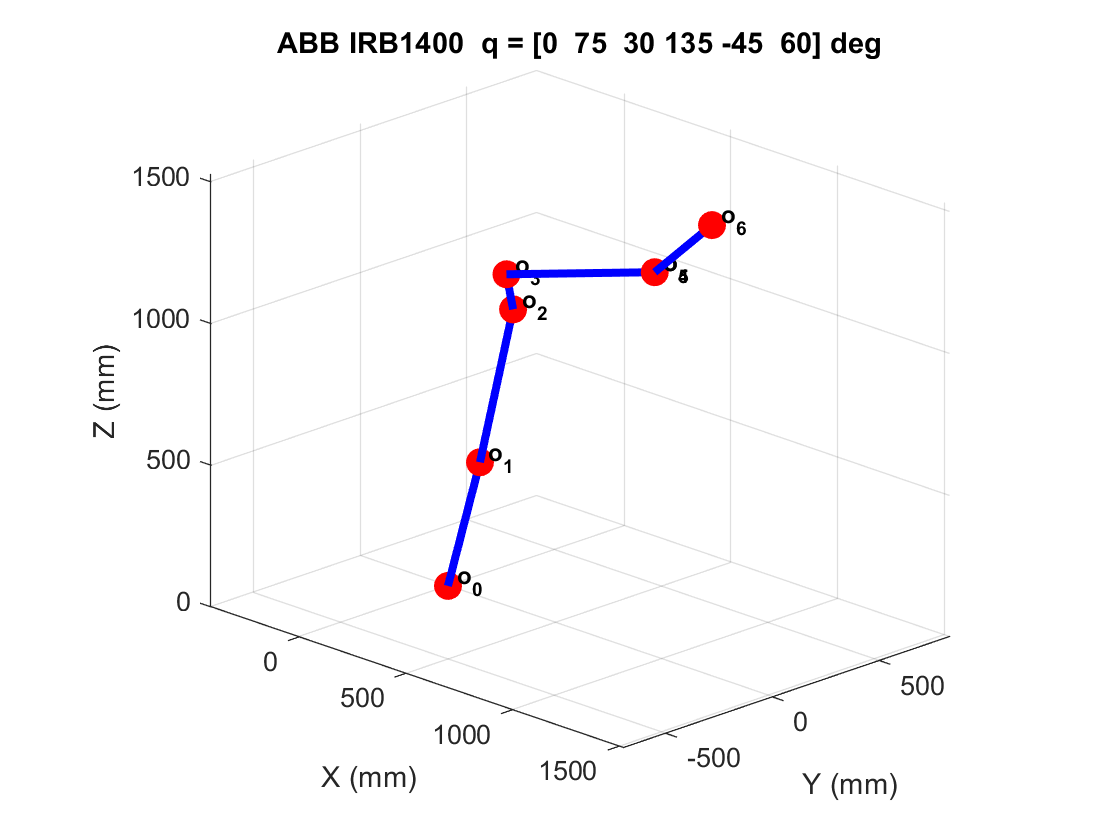
\includegraphics[width=0.75\textwidth]{robot_plot.png}
    \caption{ABB IRB1400 at
    $[\theta_1,\ldots,\theta_6] = [0^\circ,\,75^\circ,\,30^\circ,\,135^\circ,\,-45^\circ,\,60^\circ]$}
    \label{fig:robot_plot}
\end{figure}

%-------------------------------------------------------------
\subsection{Question 7 (Extra Credit): Animated Motion to Target Pose}

The following MATLAB script animates the robot moving from its home
position $[0,0,0,0,0,0]^\circ$ to the target configuration
$[0, 75, 30, 135, -45, 60]^\circ$ by linearly interpolating the joint
angles and redrawing the robot at each intermediate step.

\begin{lstlisting}[language=Matlab,
    caption={animate\_irb1400.m -- robot motion animation}]
function animate_irb1400(q_start, q_end, n_frames, save_gif)
    % Animates the ABB IRB1400 moving from q_start to q_end.
    % Inputs:
    %   q_start  -- initial joint config [q1..q6] in degrees
    %   q_end    -- target  joint config [q1..q6] in degrees
    %   n_frames -- number of interpolation steps (default: 50)
    %   save_gif -- true/false, whether to save as GIF (default: false)

    if nargin < 3; n_frames = 50; end
    if nargin < 4; save_gif = false; end

    gif_filename = 'irb1400_animation.gif';

    fig = figure;
    fig.Color = 'white';

    for k = 1:n_frames
        alpha = (k - 1) / (n_frames - 1);
        q = q_start + alpha * (q_end - q_start);

        [~, frames] = fk_irb1400(q);
        n = length(frames);
        positions = zeros(3, n);
        for i = 1:n
            positions(:, i) = frames{i}(1:3, 4);
        end

        clf;
        hold on; grid on; axis equal;
        xlabel('X (mm)'); ylabel('Y (mm)'); zlabel('Z (mm)');
        title(sprintf('Frame %d/%d  |  q = [%s] deg', ...
              k, n_frames, num2str(round(q), '%d ')));
        view(45, 20);
        xlim([-500, 1600]); ylim([-800, 800]); zlim([-300, 1800]);

        plot3(positions(1,:), positions(2,:), positions(3,:), ...
              'b-', 'LineWidth', 3);
        plot3(positions(1,:), positions(2,:), positions(3,:), ...
              'ro', 'MarkerSize', 10, 'MarkerFaceColor', 'r');

        T_ee = frames{end};
        origin = T_ee(1:3, 4);
        scale  = 80;
        colors = {'r', 'g', 'b'};
        for ax = 1:3
            dir = T_ee(1:3, ax) * scale;
            quiver3(origin(1), origin(2), origin(3), ...
                    dir(1), dir(2), dir(3), 0, ...
                    'Color', colors{ax}, 'LineWidth', 2, ...
                    'MaxHeadSize', 0.5);
        end

        labels = {'o_0','o_1','o_2','o_3','o_4','o_5','o_6'};
        for i = 1:n
            text(positions(1,i)+20, positions(2,i)+20, ...
                 positions(3,i)+20, labels{i}, ...
                 'FontSize', 8, 'FontWeight', 'bold');
        end

        drawnow;

        % --- GIF saving ---
        if save_gif
            frame     = getframe(fig);        % capture current figure
            im        = frame2im(frame);      % convert to RGB image
            [imind, cm] = rgb2ind(im, 256);   % convert to indexed color

            if k == 1
                % First frame: create the file
                imwrite(imind, cm, gif_filename, 'gif', ...
                        'Loopcount', inf, ...   % loop forever
                        'DelayTime', 0.04);     % seconds per frame
            else
                % Subsequent frames: append to file
                imwrite(imind, cm, gif_filename, 'gif', ...
                        'WriteMode', 'append', ...
                        'DelayTime', 0.04);
            end
        end

        pause(0.04);
    end

    if save_gif
        fprintf('GIF saved to: %s\n', gif_filename);
    end
    disp('Animation complete.');
end

% ---- Run and save ----
q_home   = [0,  0,  0,   0,   0,  0];
q_target = [0, 75, 30, 135, -45, 60];
animate_irb1400(q_home, q_target, 60, true);
\end{lstlisting}

\newpage
%=============================================================
\section{Part 2: ROS 2 Node -- Forward Kinematics}

\subsection{Overview}

This package implements a ROS~2 node (\texttt{fk\_node}) that
subscribes to the \texttt{/joint\_angles} topic carrying a
\texttt{Float32MultiArray} message with six values
$[q_1, q_2, q_3, q_4, q_5, q_6]$ in degrees.
Upon receiving a message, the node computes the forward kinematics
of the ABB IRB1400 using the D-H parameters from Part~1, then prints
the end-effector position and orientation matrix to the terminal.

\subsection{Package Structure}

\dirtree{%
    .1 irb1400\_fk/.
    .2 irb1400\_fk/.
    .3 \_\_init\_\_.py.
    .3 fk\_node.py.
    .2 package.xml.
    .2 setup.py.
    .2 setup.cfg.
    .2 resource/.
    .3 irb1400\_fk.
}

\subsection{Node Implementation}

\begin{lstlisting}[language=Python,
    caption={fk\_node.py -- ROS 2 forward kinematics node}]
import rclpy
from rclpy.node import Node
from std_msgs.msg import Float32MultiArray
import numpy as np

class FKNode(Node):
    def __init__(self):
        super().__init__('irb1400_fk')

        # Subscribe to /joint_angles (Float32MultiArray: [q1..q6] in degrees)
        self.subscription = self.create_subscription(
            Float32MultiArray,
            'joint_angles',
            self.listener_callback,
            10)

        self.get_logger().info('IRB1400 FK node started.')
        self.get_logger().info(
            'Waiting for joint angles [q1..q6] in degrees...')

    # ------------------------------------------------------------------ #
    def dh_matrix(self, theta_deg, d, a, alpha_deg):
        """
        Compute the standard DH transformation matrix.
        Parameters: theta, alpha in degrees; d, a in mm.
        """
        theta = np.radians(theta_deg)
        alpha = np.radians(alpha_deg)
        ct, st = np.cos(theta), np.sin(theta)
        ca, sa = np.cos(alpha), np.sin(alpha)
        return np.array([
            [ct, -st*ca,  st*sa, a*ct],
            [st,  ct*ca, -ct*sa, a*st],
            [ 0,     sa,     ca,    d],
            [ 0,      0,      0,    1]
        ])

    # ------------------------------------------------------------------ #
    def forward_kinematics(self, q):
        """
        Compute FK for the ABB IRB1400 using standard DH convention.
        Input:  q   -- list of 6 joint angles in degrees
        Output: 4x4 homogeneous transformation matrix H = T6^0
        """
        # DH table: (theta_i, d_i mm, a_i mm, alpha_i deg)
        dh_params = [
            (q[0], 475, 150,  90),  # Joint 1: base yaw
            (q[1],   0, 600,   0),  # Joint 2: shoulder pitch
            (q[2],   0, 120,  90),  # Joint 3: elbow pitch
            (q[3], 720,   0, -90),  # Joint 4: wrist roll
            (q[4],   0,   0,  90),  # Joint 5: wrist pitch
            (q[5], 255,   0,   0),  # Joint 6: wrist yaw + EE
        ]
        T = np.eye(4)
        for theta, d, a, alpha in dh_params:
            T = T @ self.dh_matrix(theta, d, a, alpha)
        return T

    # ------------------------------------------------------------------ #
    def listener_callback(self, msg):
        """Receive joint angles, compute FK, and print result."""
        # Validate message length
        if len(msg.data) != 6:
            self.get_logger().error(
                f'Expected 6 joint angles, got {len(msg.data)}')
            return

        q = list(msg.data)

        # Compute forward kinematics
        H = self.forward_kinematics(q)

        # Extract position vector (mm) and rotation matrix
        pos = H[:3, 3]
        R   = H[:3, :3]

        # Print end-effector pose to terminal
        self.get_logger().info(
            f'\nReceived joints (deg): {[round(qi,2) for qi in q]}\n'
            f'  Position (mm):\n'
            f'    x = {pos[0]:.2f}\n'
            f'    y = {pos[1]:.2f}\n'
            f'    z = {pos[2]:.2f}\n'
            f'  Rotation matrix R_6^0:\n'
            f'    [{R[0,0]:7.4f}  {R[0,1]:7.4f}  {R[0,2]:7.4f}]\n'
            f'    [{R[1,0]:7.4f}  {R[1,1]:7.4f}  {R[1,2]:7.4f}]\n'
            f'    [{R[2,0]:7.4f}  {R[2,1]:7.4f}  {R[2,2]:7.4f}]'
        )

# ---------------------------------------------------------------------- #
def main(args=None):
    rclpy.init(args=args)
    node = FKNode()
    rclpy.spin(node)
    node.destroy_node()
    rclpy.shutdown()

if __name__ == '__main__':
    main()
\end{lstlisting}

\subsection{How to Run}

Build and source the package:
\begin{verbatim}
cd ~/ros2_ws
colcon build --packages-select irb1400_fk
source install/setup.bash
\end{verbatim}

Launch the node:
\begin{verbatim}
ros2 run irb1400_fk fk_node
\end{verbatim}

Publish joint angles from the terminal (six test cases):
\begin{verbatim}
# Test 1: Home position (all zeros)
ros2 topic pub --once /joint_angles std_msgs/msg/Float32MultiArray \
  "data: [0.0, 0.0, 0.0, 0.0, 0.0, 0.0]"

# Test 2: Question-5 configuration
ros2 topic pub --once /joint_angles std_msgs/msg/Float32MultiArray \
  "data: [0.0, 75.0, 30.0, 135.0, -45.0, 60.0]"

# Test 3: Shoulder 90 deg
ros2 topic pub --once /joint_angles std_msgs/msg/Float32MultiArray \
  "data: [0.0, 90.0, 0.0, 0.0, 0.0, 0.0]"

# Test 4: Base rotated 90 deg
ros2 topic pub --once /joint_angles std_msgs/msg/Float32MultiArray \
  "data: [90.0, 0.0, 0.0, 0.0, 0.0, 0.0]"

# Test 5: Elbow and wrist active
ros2 topic pub --once /joint_angles std_msgs/msg/Float32MultiArray \
  "data: [45.0, 45.0, 45.0, 0.0, 0.0, 0.0]"

# Test 6: All joints active
ros2 topic pub --once /joint_angles std_msgs/msg/Float32MultiArray \
  "data: [30.0, 60.0, -30.0, 90.0, -60.0, 45.0]"
\end{verbatim}

\subsection{Results}

\begin{figure}[h]
    \centering
    \begin{minipage}{0.54\textwidth}
        \centering
        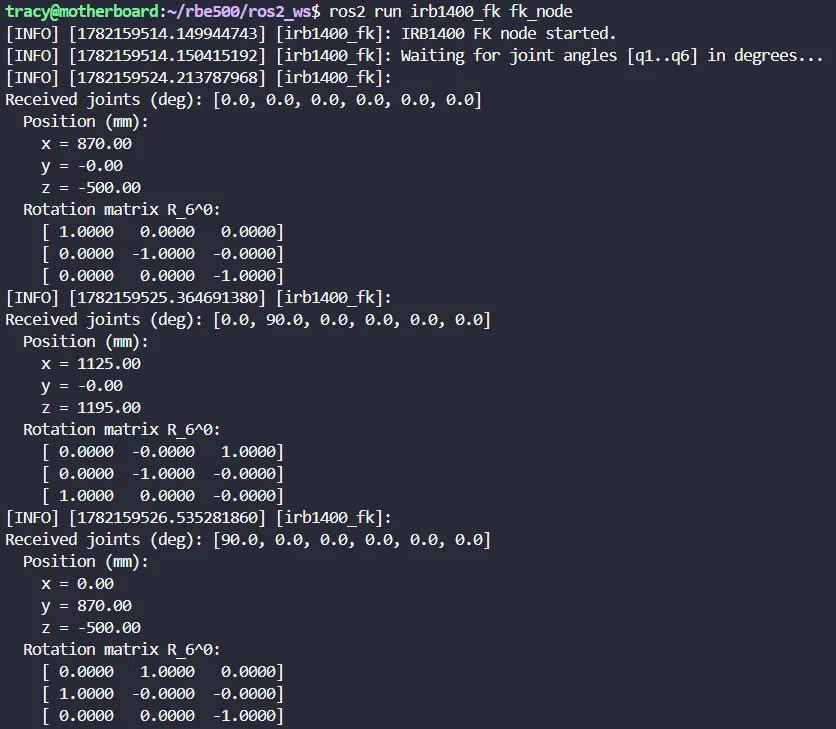
\includegraphics[width=\textwidth]{fk_terminal_output_1.png}
    \end{minipage}
    \hfill
    \begin{minipage}{0.4\textwidth}
        \centering
        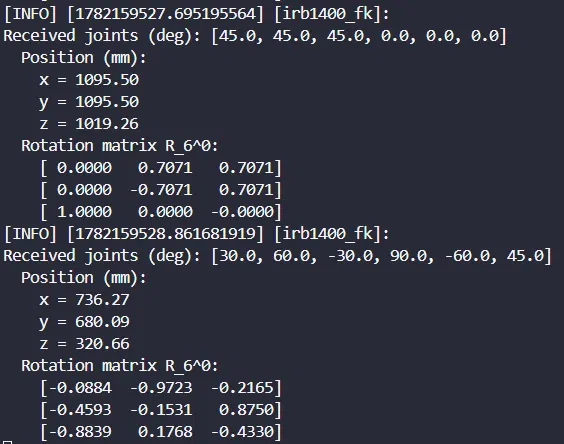
\includegraphics[width=\textwidth]{fk_terminal_output_2.png}
    \end{minipage}
    \caption{Terminal output showing FK results for all six test cases.
    \textit{Left:} Tests 1--3 (home, shoulder $90^\circ$, base $90^\circ$).
    \textit{Right:} Tests 4--5 (elbow/wrist, all joints active).}
    \label{fig:fk_output}
\end{figure}

\end{document}